\documentclass[12pt]{article}

\usepackage{sbc-template}
\usepackage{graphicx,url}
\usepackage[utf8]{inputenc}
\usepackage[brazil]{babel}
\usepackage[utf8]{inputenc}  
\usepackage{xcolor}
\usepackage{multirow}
\usepackage{amsfonts}

\sloppy

\title{Árvores B e B\nolinebreak+ em Busca de Gravações de Música Clássica\\}

\author{Caio Stoduto\inst{1}, Lucas Guido\inst{1}, Nicolas Greco\inst{1},\\
Paulo Bezerra\inst{1}, Stephania Ferreira\inst{1}, Tales Bartolome\inst{1}}

\address{CMCC -- Universidade Federal do ABC (UFABC)\\
  Santo André -- SP -- Brazil
  \email{\{caio.stoduto,lucas.guido\}@aluno.ufabc.edu.br} \vspace{-1em}
  \email{\{nicolas.greco,paulo.bezerra\}@aluno.ufabc.edu.br} \vspace{-1em}
  \email{\{stephania.ferreira,m.bartolome\}@aluno.ufabc.edu.br} }

\begin{document} 

\maketitle

\begin{abstract}
  This meta-paper describes the style to be used in articles and short papers
  for SBC conferences. For papers in English, you should add just an abstract
  while for the papers in Portuguese, we also ask for an abstract in Portuguese
  (``resumo''). In both cases, abstracts should not have more than 10 lines and
  must be in the first page of the paper.
\end{abstract}
     
\begin{resumo} 
  Este meta-artigo descreve o estilo a ser usado na confecção de artigos e
  resumos de artigos para publicação nos anais das conferências organizadas pela
  SBC. É solicitada a escrita de resumo e abstract apenas para os artigos
  escritos em português. Artigos em inglês deverão apresentar apenas abstract.
  Nos dois casos, o autor deve tomar cuidado para que o resumo (e o abstract)
  não ultrapassem 10 linhas cada, sendo que ambos devem estar na primeira página
  do artigo.
\end{resumo}

\section{Introdução}
Dentro da música clássica, peças canônicas são gravadas centenas de vezes e,
para grande parte dos ouvintes, a escuta atenta de diferentes gravações é um
processo importante, permitindo a comparação das nuances de cada gravação~\cite{Bl:25}.
Assim, um sistema que permita a busca de gravações de uma música é essencial.
No entanto, como apontado por Blakeley~\cite{Bl:25}, os serviços de \emph{streaming},
que permitem acesso instantêneo e ilimitado a um grande catálogo de músicas, não
possuem funcionalidades focadas em pesquisa de música clássica, tendo como foco
maior a música popular.
Assim sendo, a busca de música clássica nestes serviços é difícil e imprecisa, 
além de possuírem uma interface que não está alinhada a este estilo.
Por causa disso, as necessidades dos ouvintes de música clássica não são supridas
pelos grandes serviços de \emph{streaming}, como Spotify, Deezer e Youtube Music.

Tendo isso em vista, serviços dedicados à música clássica, tais como
IDAGIO, Apple Music Classical e Presto Music, foram criados e permitem busca
especializada, separando músicas de gravações, e interface considerando esta
divisão~\cite{Bl:25}.
Apesar de isto representar um avanço, a quantidade de plataformas ainda é pequena
e muitas delas ainda não estão bem estabelecidas, pois é um mercado nichado, e 
não há alternativas de código aberto, todas são iniciativas privadas e sem
detalhes acerca da implementação~\cite{Bl:25}.

Com base nisso, este trabalho objetiva implementar uma base de dados dedicada
para busca de peças de música clássica, de modo a permitir acesso mais
descentralizado a um sistema de busca, visando impulsionar o desenvolvimento de
novas soluções para este problema.
Para isso, serão utilizadas árvores B e B+ para a organização das informações,
pois estas são algumas das principais estruturas usadas no armazenamento de
informações em memória secundária~\cite{Co:79}.

O restante do artigo está organizado da seguinte forma:
a Seção~\ref{sec:revisao} apresenta informações sobre as árvores B e B+ e
trabalhos relacionados ao tema de pesquisa, a Seção~\ref{sec:problem} apresenta
em mais detalhes o problema de pesquisa. A Seção~\ref{sec:implementation}
descreve a implementação e as decisões tomadas para tal. A Seção~\ref{sec:results}
apresenta os resultados obtidos sobre a eficiência das implementações.
Por fim, a Seção~\ref{sec:conclusion} conclui o trabalho, com considerações
gerais e possibilidades de trabalhos futuros de modo a melhor explorar a temática.



\section{Revisão Bibliográfica} \label{sec:revisao}
Esta seção apresenta a fundamentação teórica das estruturas de dados utilizadas,
bem como outros trabalhos relacionados ao tema do presente artigo.

\subsection{Fundamentação Teórica}
Tendo em vista o uso de árvores B neste trabalho, esta seção tem como objetivo 
apresentar esta estrutura, sua utilidade e alguns resultados essenciais.

Durante o processo de manutenção de uma base de dados, um dos maiores custos
operacionais é o de acesso à memória secundária.
O acesso à memória secundária toma um tempo de ordens de magnitude maior do que
o tempo que o processador leva em instruções simples como de comparação de valores.
No entanto, diversas aplicações trabalham com uma quantidade de dados muito maior
do que a capacidade da memória principal financeiramente viável, o que torna o
acesso ao disco uma operação fundamental para o processamento de qualquer base
de dados e, ao pensarmos na otimização de tal processamento, a diminuição da
quantidade destes acessos ao disco pode se tornar o principal fator para o ganho
de performance operacional~\cite{clrs:22}.

Uma das soluções mais usadas para otimizar operações em memória secundária é o
uso de árvores B e suas variantes~\cite{Co:79}. Estas estruturas são árvores
nas quais cada nó pode armazenar mais que um registro, diferentemente das
árvores binárias.

Elas são definidas de modo que, considerando uma árvore não vazia de ordem
$d \in \mathbb{N}$, a raiz seja uma folha ou tenha no mínimo dois filhos, cada
nó diferente da raiz e das folhas possua entre $d+1$ e $2d +1$ filhos e todas as
folhas estejam no mesmo nível.
Além disso, pode-se concluir que cada nó que não é a raiz contém entre $d$ e $2d$
chaves e a altura $h$ da árvore está no intervalo
\[ \log_{2d+1} (n+1) \leq h \leq 1 + \log_{d+1} \left(\frac{n + 1}{2}\right)~\cite{SwMa:10}. \]

A característica de altura logarítmica se mostra muito importante, pois faz com
que operações de inserção e busca também tenham custo logarítimico.
Ademais, a possibilidade de armazenar diversas chaves em cada nó é adequada para
armazenamento em memória secundária pois possibilita tratar um nó como uma página % XXX o que é uma página?
em disco, de modo que a quantidade de leituras em memória secundária é minimizada~\cite{Kn:98}.

% Como apontado por Comer em seu artigo de 1979 \cite{Co:79}, a árvore B é uma
% estrutura de dados utilizada para a organização de um arquivo e os índices
% (também chamados chaves) de seus registros. Além disso, é uma generalização das
% árvores binárias balanceadas. No entanto, diferente das árvores binárias, cada
% nó de uma árvore B de ordem $t$ contém $n \in \mathbb{N}$ chaves, onde $t \le n
% \le 2t-1$, além de $n+1$ ponteiros por nó. Em consequência, o custo para
% as operações de busca, inserção e remoção crescem em proporção logarítmica com o
% aumento de registros do arquivo, o que representa um custo operacional
% relativamente baixo~\cite{Co:79}.

% Para acessar cada nó da árvore B, é necessário acessar a memória secundária.
% Apesar disso, seguindo as regras que definem a estrutura da árvore e seu
% balanceamento, em cada acesso é recuperado da memória não um registro, mas uma
% página de registros, de modo a se atingir uma pequena quantidade de acessos ao
% disco e a otimização dos processos de manipulação de registros do arquivo.

Já a árvore B+ é uma variação da árvore B, possuindo como
diferencial a ausência de registros em nós não-folha da estrutura, ou seja,
os registros estão contidos apenas nas folhas e as chaves estarão nos nós internos,
tendo um papel de guia na busca efetuada na árvore.
Além disso, os nós folha da árvore são ligados, de modo que é possível percorrer
os registros armazenados na árvore sequencialmente~\cite{Pm:10}.


\subsection{Trabalhos Relacionados}

A indexação de pesquisas é um problema amplamente discutido em artigos ao longo
das décadas por conta de suas aplicabilidades no uso dos computadores,
principalmente com a emersão dos serviços de busca e \emph{streaming}.

O artigo "Music search engines: Specifications and challenges" discute como
aborda o crescente campo de pesquisa dos motores de busca de música (\emph{Music
Search Engines}), motivado pelo crecimento exponencial da quantidade de músicas
disponíveis na internet e publicadas diariamente. Os autores abordam as
principais funcionalidades.


{\color{red}Existem muitos estudos focados no desenvolvimento de métodos de indexação
e no desenvolvimento de mecanismos eficientes de busca de músicas, que já são
aplicados de acordo com determinados critérios.} Alguns dos critérios comuns,
que são relativamente antigos mas perpetuados na busca em serviços de \emph{streaming}
da atualidade, são evidenciados por  Nanopoulos et al. em seu artigo de 2009 \cite{NaRaRuMa:09}. Nele, é
dissertado sobre diferentes formas de realizar a busca por música em alguns
serviços como Allmusic, Yahoo!Music, iTunes e entre outros. Dentre elas,
pode-se apontar a busca por metadados relacionados a músicas (biografia de
artista, novos lançamentos, análises e entre outros), através de letra de música
e, para aumentar o leque musical de um ouvinte, há a recomendação de músicas
similares a escutadas e geração de playlists automáticas. As duas formas
apontadas de busca são por texto, por meio dos metadados, ou “smart words”, que
associam a músicas para certas ocasiões (músicas para ouvir no carro ou músicas
alegres) ou característica de voz de tal artista ou a tags, ou busca por áudio,
que nos serviços da atualidade não são muito utilizados.

Na atualidade, os serviços de \emph{streaming} de música, como indicado Li et al. no seu
artigo de 2019 \cite{LiThChToGa:19}, os mecanismos de busca, para manter certa qualidade precisam
balancear o específico do abrangente, em que dependendo do indivíduo que irá
pesquisar, ele terá uma mentalidade diferente no que deseja, que, de acordo com o artigo
mencionado, pode ser dividida em dois grupos: focada e não focada. O usuário com
a mente focada, ao efetuar uma busca, procura algo em particular, que seria agregado com o projeto, em
especificidade no gênero de música clássica, enquanto o não focado possui uma
ideia vaga do que busca, estando aberto a sugestões, efetuando pesquisas com frases mais subjetidas,
como apresentada por Nanopoulos et al. Diante disso, é mostrado a
necessidade da caracterização destes grupos e como cada usuário se enquadra em
cada um ou seus hábitos dependendo do meio que é inserido, desde gastar mais
tempo em uma busca ou não, onde a implementação de árvores B e B + está sendo
voltada ao estilo de busca específica, focada.



\section{Problema de Pesquisa} \label{sec:problem}

Levando em consideração o contexto de músicas clássicas, uma composição, feita
por um único compositor, possui diversas interpretações por diferentes músicos.
Com isso, uma necessidade relevante para os ouvintes desse estilo de música é a
busca dessas diferentes interpretações de uma composição de forma prática e
amigável, elevando a experiência do usuário.

Mesmo com isso em mente, poucas plataformas de \emph{streaming} de música levam
isso em consideração, pois se trata de um nicho dentro da imensa diversidade de
usuários, estilos e gêneros musicais.
Como exemplo, o comportamento do Spotify, uma das principais plataformas de
\emph{streaming} de música, não é adequado, pois, ao realizar uma pesquisa com o
nome da composição desejada, são exibidos resultados irrelevantes, como outras
músicas com nomes parecidos (tanto do mesmo compositor, como de outros), 
dificultando a busca por gravações da peça desejada.
A Figura~\ref{fig:spotify}, na qual foi feita a pesquisa ``Bach Trio Sonata no. 3'',
é um exemplo disso, pois nenhum dos resultados principais condiz com a música
pesquisada.

\begin{figure}[ht]
\centering
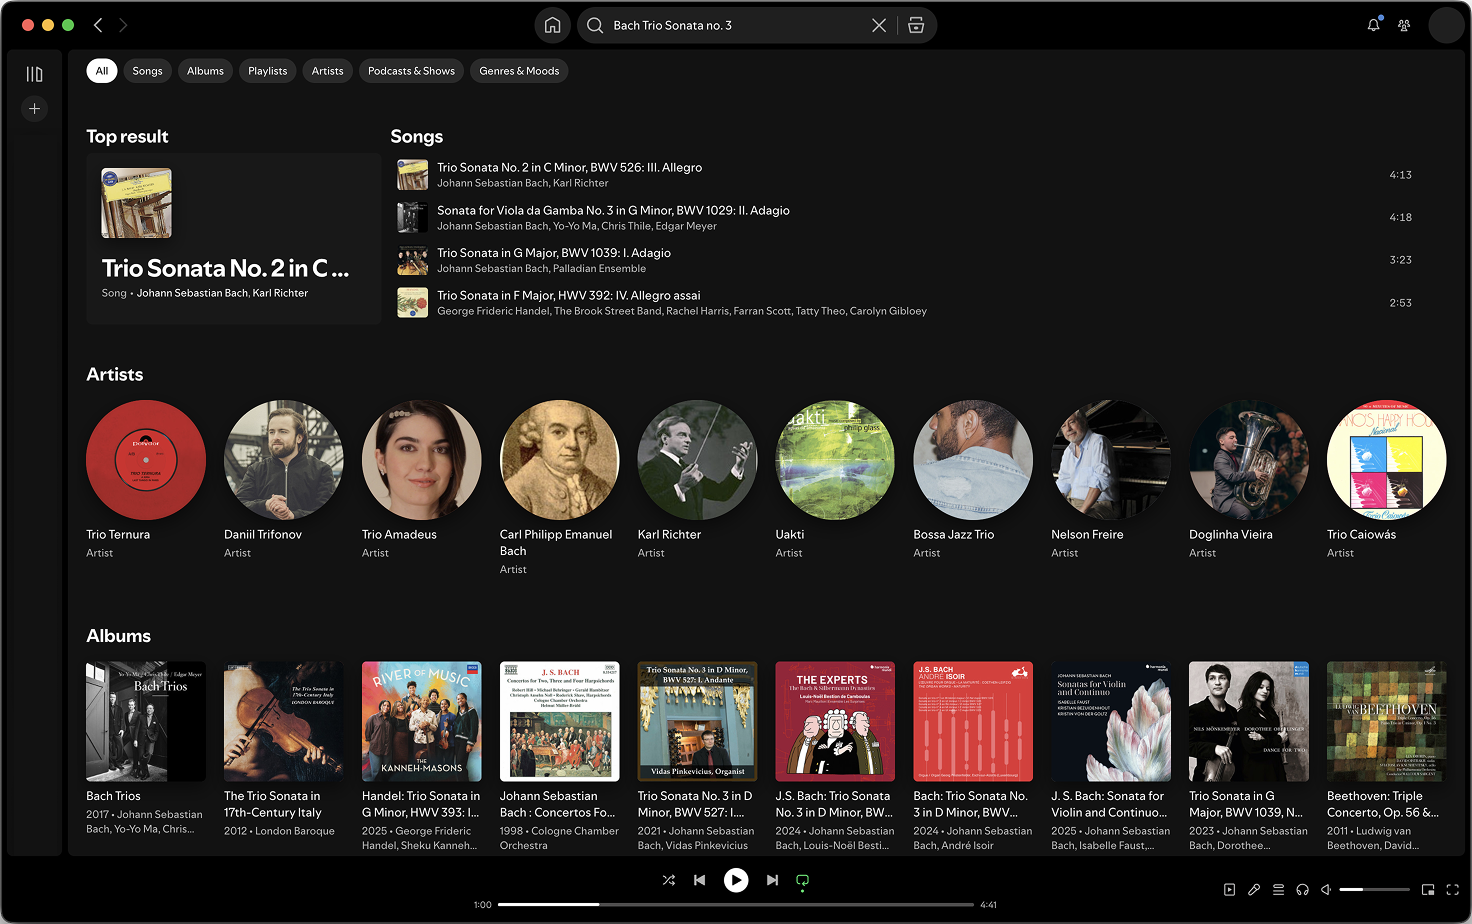
\includegraphics[width=1\textwidth]{figuras/Spotify.png}
\caption{Resultado de busca na plataforma Spotify}
\label{fig:spotify}
\end{figure}

Em contrapartida, existem plataformas de \emph{streaming} especializadas em
música clássica, como a plataforma IDAGIO e Presto Music, que adaptam seu
algoritmo de pesquisa especificamente para este nicho. Apesar disso, por se
tratar de um nicho limitado, há a grande iminência de um monopólio, por
existirem um número baixo de plataformas com funcionalidades voltadas para
ouvintes de música clássica. O principal exemplo desse movimento foi a aquisição
da antiga Primephonic pela Apple, criando a Apple Music Classical. Com isso,
abre-se o debate de se uma empresa privada com alcance de usuários diversificado
manteria a qualidade do serviço tendo em mente ser uma empresa privada que visa
primariamente o lucro, onde uma possível queda de ouvintes poderia tender a
abolição dessas funcionalidades e do desenvolvimento desse setor.

Dado o exposto, este artigo cria uma implementação na seção seguinte de uma aplicação
computacional com o intuito de expandir o acesso a algoritmos especializados para busca
de músicas clássicas, respeitando a necessidade explicitada anteriormente, por
meio de uma prova de conceito. Isso implica a liberdade de qualquer usuário
poder usar a solução de código livre disponibilizada podendo adaptar às próprias
necessidades, como o uso em plataformas de \emph{streaming} ou em arquivos
locais. Além disso, possibilita a adoção desse sistema ou guia para criação de um sistema
próprio por empresas já estabelecidas neste mercado
para uma disponibilidade de funcionalidades mais
ampla dentre as plataformas, que resulta em refinamento nos seus mecanismos de busca e redução
da concentração destes sistemas em poucos serviços.

\section{Implementação} \label{sec:implementation}

A implementação baseia-se na ideia de uma árvore de busca para o indexamento de
músicas clássicas, permitindo a obtenção de todas as gravações pelo termo de
busca, ou seja, o nome da composição. Para o desenvolvimento do sistema, foram
utilizadas duas alternativas de estruturas de dados semelhantes, as árvores B e
B\nolinebreak+ persistentes, permitindo que crie-se uma comparação direta entre
a eficiência em termos de complexidade de tempo, espaço e facilidade de
implementação.

Considerando a implementação, a estrutura de dados dentro das árvores B e
B\nolinebreak+ são usadas para guardar valores e registros. Com isso, o registro
guarda as seguintes informações:
\begin{itemize}
  \item Compositor (ex.: Ludwig van Beethoven);
  \item Nome da composição (ex.: Sinfonia no. 9);
  \item Catálogo (ex.: op. 125);
\end{itemize}

Além dessa estrutura, os metadados da música também compõem a própria chave,
sendo esta composta pela concatenação do Compositor e do Catálogo (ex:
"Ludwig van Beethoven125"). Com isso, o principal valor de busca presente no
valor dos elementos da árvore é o nome da composição. Com isso, a árvore serve
como um indexamento de dados atrelados a um conjunto de gravações, cabendo o
acréscimo de informações de outros tipos de metadados, como duração média,
quantidade de gravações, etc.

Além disso, é criado dinâmicamente um arquivo único para cada composição que
contém uma listagem sequencial de todas as gravações dessa composição
analisadas. Esse arquivo é armazenado na memória secundária com o caminho
atrelado aos metadados armazenados na árvore. A decisão da sequencialidade do
arquivo digital justifica-se pelo objetivo final da listagem de todas as
gravações, simplificando a implementação do projeto.

Com a problemática em mente, foi decidida a implementação do programa utilizando
a linguagem C++, pois ela apresenta um conjunto de características
imprescindíveis para o projeto. A principal característica é sua alta
performance, provindo da sua natureza de compilação \emph{Ahead-of-Time} (AOT).
O quesito de tempo de execução é essencial para o projeto, já que o propósito é
uma ferramenta eficiente de busca. Outra característica da linguagem que
facilita a implementação é sua vasta quantidade de bibliotecas que incorporam
partes essenciais do código elaborado neste artigo.

As duas bibliotecas utilizadas foram o Tipo Abstrato de Dados (TAD) da árvore
B+\footnote{\url{https://github.com/ByJuanDiego/disk-b-plus-tree}} e a
biblioteca TagLib\footnote{\url{https://taglib.org/}}, para a leitura de
metadados de arquivos de música. Isso resultou numa implementação mais simples,
garantindo um código conciso e bem estruturado.

\section{Resultados} \label{sec:results}
As árvores B e B\nolinebreak+ são úteis quando o conjunto de dados de consulta é
grande suficiente para não caber por completo na memória principal e precisa ser
acessado da memória secundária. Elas agem de maneira a buscar o menor número de
acessos ao disco para acessar efetivamente o registro requisitado. A altura
dessa estrutura de árvores está no intervalo de $[\log_{2t-1} (n+1),\ \log_t
\frac{n + 1}{2}]$, onde $t$ é a ordem da árvore que indica a quantidade mínima
de registros armazenados em um nó e $n$ a quantidade de elementos
\cite{clrs:22}. Com isso, a quantidade de acessos a páginas do disco é de
complexidade $O(\log_t n)$, entretanto, demora o tempo $O(t)$ para percorrer os
registros dentro de cada nó, compondo no final a complexidade de $O(t \log_t n)$
para buscas~\cite{clrs:22,Pm:10}. Por isso, são parte integrante da estrutura
central do projeto, pois permitem a indexação eficiente de cada composição a
partir de uma chave de identificação única, representado na
Tabela~\ref{tab:complexidades}.

\begin{table}[ht]
\centering
\caption{Tabela de Complexidades das Árvores B e B\nolinebreak+}
\label{tab:complexidades}
\begin{tabular}{|c|c|c|}
\hline
  Estrutura & Operação & Complexidade \\ \hline
  \multirow{4}{*}{Árvore B} & Espaço   & $O(n)$ \\
  \cline{2-3} & Busca    & $O(t \log_t n)$ \\
  \cline{2-3} & Inserção & $O(t \log_t n)$ \\
  \cline{2-3} & Remoção  & $O(t \log_t n)$ \\
  \hline
  \multirow{4}{*}{Árvore B\nolinebreak+} & Espaço & $O(n)$ \\
  \cline{2-3} & Busca & $O(t \log_t n)$ \\
  \cline{2-3} & Inserção & $O(t \log_t n)$\\
  \cline{2-3} & Remoção & $O(t \log_t n)$\\
  \hline
\end{tabular}
\end{table}


\section{Conclusão} \label{sec:conclusion}



\bibliographystyle{sbc}
\bibliography{bibliography}

\end{document}
